\documentclass{beamer}

\mode<presentation>
{ \usetheme{CambridgeUS} }
\setbeamersize{text margin left=0.75cm}

\AtBeginSection[]
{
   \begin{frame}
       \frametitle{Outline}
       \tableofcontents[currentsection]
   \end{frame}
}

\usepackage{graphicx}
\usepackage{textcomp}
\usepackage{tikz}

\title{Git}
\author{Nelson Elhage\and Anders Kaseorg}
\institute[SIPB]{Student Information Processing Board}
\date{October 21, 2008}

\newcommand{\sh}[1]{\$ {\color{beamer@blendedblue}#1}}

\begin{document}

\begin{frame}
    \titlepage
\end{frame}

\section{The Git model}

\begin{frame}
  \frametitle{The Git model}

  \begin{itemize}
  \item A Git repository contains four kinds of \emph{objects}.
  \item An object is either a \emph{blob} (file), a \emph{tree}
    (directory), a \emph{commit}, or a \emph{tag}.
  \item Every object is uniquely identified by a 40 hex digit number,
    which is the SHA-1 hash of its contents.
    \begin{itemize}
    \item Don't worry---identifiers can be abbreviated by truncation,
      or referenced with human-readable names.
    \end{itemize}
  \item Some objects refer to other objects using their identifiers.
  \end{itemize}
\end{frame}

\begin{frame}
  \frametitle{Objects}

  \begin{itemize}
  \item A blob object is a file's contents.
  \item A tree object is a directory---a list of zero or more
    directory entries, each of which has
    \begin{itemize}
    \item a \emph{name}
    \item a UNIX \emph{mode}
    \item a tree id or blob id
    \end{itemize}
  \item A commit object contains
    \begin{itemize}
    \item a tree id
    \item zero or more \emph{parents}, which are commit ids
    \item an \emph{author} (name, email, date)
    \item a \emph{committer} (name, email, date)
    \item a \emph{log message}
    \end{itemize}
  \item A tag object contains
    \begin{itemize}
    \item a \emph{tag name}
    \item a \emph{tagger} (name, email, date)
    \item a reference to another object (usually a commit)
    \item an optional \emph{log message}
    \end{itemize}
  \end{itemize}
\end{frame}

\begin{frame}
  \frametitle{A commit}
  \hspace*{-0.5cm}\includegraphics[width=12cm]{commit}
\end{frame}

\begin{frame}
  \frametitle{More commits}
  \hspace*{-0.5cm}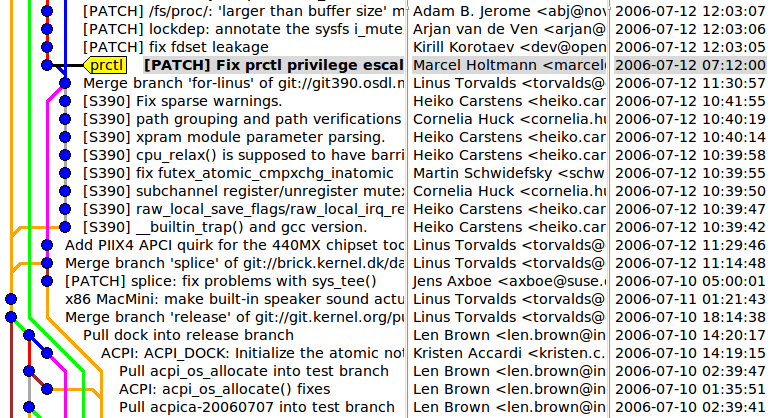
\includegraphics[width=12cm]{prctl}
\end{frame}

\begin{frame}
  \frametitle{A Git repository}
  \begin{itemize}
  \item A Git repository is a collection of
    \emph{refs}---\emph{branches} and \emph{tags}.  (Branches are also
    known as \emph{heads}.)
  \item A ref is a named mutable pointer to an object (usually a
    commit).
    \begin{itemize}
    \item \texttt{HEAD} $\to$ \texttt{refs/heads/master}
    \item \texttt{refs/heads/master} $\to$ \texttt{commit fec6ed\ldots}
    \item \texttt{refs/heads/ftrace} $\to$ \texttt{commit ce5c1e\ldots}
    \item \texttt{refs/tags/v2.6.8} $\to$ \texttt{commit e8ce2f\ldots}
    \item \texttt{refs/tags/v2.6.27} $\to$ \texttt{tag 4b5127\ldots}
    \end{itemize}
  \item The repository automatically stores the directed acyclic graph
    of objects rooted at these refs.
  \end{itemize}
\end{frame}

\begin{frame}
  \frametitle{Branches}

  \begin{itemize}
  \item Git was designed to enable lightweight branching and merging.
  \item Each repository can have any number of branches.
  \item Branches are just refs---pointers into the DAG of
    commits---and these pointers themselves are not versioned.
    \begin{itemize}
    \item So you don't need to be afraid of making throwaway branches
      for experiments.
    \end{itemize}
  \end{itemize}
\end{frame}

\begin{frame}
  \frametitle{Consequences of the Git model}

  \begin{itemize}
  \item Git tracks the history of your whole project, not the history
    of individual files.
    \begin{itemize}
    \item Best practice is to keep projects that are logically
      separate in separate Git repositories.
    \end{itemize}
  \item Git does not track renames as metadata in the repository.
    \begin{itemize}
    \item Instead, renames are automatically detected based on content
      when this information is needed.
    \end{itemize}
  \item A commit ID cryptographically certifies the integrity of the
    \emph{entire history} of the repository up to that commit.
    \begin{itemize}
    \item Git has powerful tools for rewriting history---but this
      requires communication with everyone that has pulled any
      affected commits from your repository.
    \end{itemize}
  \end{itemize}
\end{frame}

\section{Using Git}

\begin{frame}
  \frametitle{Getting a Git repository}

  \begin{description}[\texttt{git clone \textit{url}}]
  \item[\texttt{git init}] Create an empty Git repository in the
    current directory.  By default it will have one branch named
    \texttt{master}.
  \item[\texttt{git clone \textit{url}}] Clone the Git repository from
    \texttt{\textit{url}}.  This may be over HTTP, SSH, or the Git
    protocol, or it may be a path to another local repository.
  \end{description}

  Both of these operations will create a \emph{working copy}.
\end{frame}

\begin{frame}
  \frametitle{Working copy}
  \begin{itemize}
  \item Every working copy has its own Git repository in the
    \texttt{.git} subdirectory (with arbitrarily many branches and
    tags).
    \begin{itemize}
    \item The most important ref is \texttt{HEAD}, which refers to the
      current branch.
    \end{itemize}
  \item The \texttt{.git} subdirectory also stores the \emph{index}: a
    staging area for changes on top of \texttt{HEAD} that will become
    part of the next commit.
  \item Finally, the files outside of \texttt{.git} are the
    \emph{working tree}.
  \end{itemize}
\end{frame}

\begin{frame}
  \frametitle{Git workflow}
  \begin{itemize}
  \item Changes made to the working tree can be \emph{added} to the
    index.
  \item The index can be \emph{committed} to the current branch (where
    it will then become the new \texttt{HEAD}).
  \end{itemize}

  \begin{center}
    \includegraphics[width=9cm]{index}
  \end{center}
\end{frame}

\begin{frame}
  \frametitle{Constructing commits}
  \begin{description}[\texttt{git show \textit{object}}]
  \item[\texttt{git add \textit{file}}] Add or update
    \texttt{\textit{file}} from the working tree into the index.
  \item[\texttt{git reset \textit{file}}] Unstage changes to
    \texttt{\textit{file}} in the index, without touching the working
    copy.
  \item[\texttt{git rm \textit{file}}] Delete \texttt{\textit{file}}
    from the index and the working tree.
  \item[\texttt{git status}] Display the files changed in the index
    and in the working tree.
  \item[\texttt{git commit}] Make a commit out of the current index.
  \item[\texttt{git commit -a}] Shortcut for adding all modified files
    to the index and committing.
  \end{description}
\end{frame}

\begin{frame}
  \frametitle{Displaying changes}

  \begin{description}[\texttt{git diff --cached}]
  \item[\texttt{git log}] List the commits on the current branch.
  \item[\texttt{git show \textit{object}}] Show an object (e.g. a commit).
  \item[\texttt{git diff}] Show the differences between the index and
    the working tree.
  \item[\texttt{git diff --cached}] Show the differences between
    \texttt{HEAD} and the index.
  \item[\texttt{git diff \textit{commit}}] Show the differences
    between \textit{commit} and the working tree.
  \end{description}
\end{frame}

\begin{frame}
  \frametitle{Manipulating branches}

  \begin{description}[\texttt{git branch -d \textit{branch}}]
  \item[\texttt{git branch}] List the branches in your repository,
    with the current branch highlighted.
  \item[\texttt{git checkout \textit{branch}}] Switch to the branch
    named \texttt{\textit{branch}}.  This updates \texttt{HEAD}, the
    index, and the working tree.
  \item[\texttt{git checkout -b \textit{branch} [\textit{commit}]}]
    Create a new branch named \texttt{\textit{branch}} starting at
    \texttt{\textit{commit}} (defaulting to current \texttt{HEAD}),
    and switch to it.
  \item[\texttt{git branch -d \textit{branch}}] Delete the branch
    \texttt{\textit{branch}}.
  \item[\texttt{git branch -m \textit{oldbranch} \textit{newbranch}}]
    Rename \texttt{\textit{oldbranch}} to \texttt{\textit{newbranch}}.
  \end{description}
\end{frame}

\begin{frame}
  \frametitle{Referring to commits}

  \begin{description}[\texttt{\textit{commit}\^{}2}]
  \item[\texttt{fc8da7a06bb66b707e7f5406657d5a3b7ee42c66}] You
    can always refer to a commit by its full SHA-1 ID, but this gets
    unwieldy very quickly.
  \item[\texttt{fc8da7}] You can use a truncated SHA-1 as long as it
    is unambiguous.
  \item[\texttt{\textit{refname}}] You can refer to a branch or tag by
    name.
  \item[\texttt{\textit{commit}\^{}}] Append a \texttt{\^{}} to get
    the (first) parent of a commit.
  \item[\texttt{\textit{commit}\^{}2}] The second parent of a commit,
    etc.
  \item[\texttt{\textit{commit}\~{}4}] Short for
    \texttt{\textit{commit}\^{}\^{}\^{}\^{}}---the
    great-great-grandparent of a commit.
  \end{description}
  \dots and more (see \texttt{git help rev-parse} for a full
  description of the syntax).
\end{frame}

\begin{frame}
  \frametitle{Merging}
  \begin{description}[\texttt{git merge \textit{commit}}]
  \item[\texttt{git merge \textit{commit}}] Merge
    \texttt{\textit{commit}} into \texttt{HEAD}. The index must not
    contain any staged changes.
  \end{description}

  \begin{itemize}
  \item In the general case, this will result in a \emph{merge
      commit}---a commit with more than one parent.
    \begin{center}
      \includegraphics[width=4cm]{merge}
    \end{center}
  \item If \texttt{\textit{commit}} is an ancestor of \texttt{HEAD},
    then the merge is a no-op.
  \item If \texttt{\textit{commit}} is a descendent of \texttt{HEAD},
    then the merge degenerates into a \emph{fast-forward}.
  \end{itemize}
\end{frame}

\begin{frame}
  \frametitle{Resolving merge conflicts}

  \begin{itemize}
  \item \texttt{git merge} works roughly by creating a diff against
    the common ancestor commit, and applying it against the current
    \texttt{HEAD}.  (The general case is much more complicated.)
  \item Sometimes this patch will not apply to the current
    \texttt{HEAD}.  This situation is called a \emph{merge conflict}.
    \begin{itemize}
    \item Git will respond by inserting \emph{conflict markers} into
      the conflicted files, and asking you resolve the conflict.
    \item Don't panic!
    \item To resolve the conflict, edit the conflicted files
      appropriately and then \texttt{git add} them.
    \item Alternatively, you can run \texttt{git mergetool} to resolve
      the conflicts interactively in a graphical diff program.
    \end{itemize}
  \end{itemize}
\end{frame}

\begin{frame}[fragile]
  \frametitle{Merging example}

  \hspace*{-0.5cm}
  \begin{tikzpicture}
    \useasboundingbox (0, 0) rectangle (11.5, 7);
    \begin{scope}
      \clip (0, 0) rectangle (11.5, 7);
      \draw (0, 0) node[anchor=south west,inner sep=0pt] {\vbox{\footnotesize
\begin{semiverbatim}
\only<1->{\sh{seq 5 > numbers}
}\only<2->{\sh{git init}
Initialized empty Git repository in /tmp/foo/.git/
}\only<3->{\sh{git add numbers}
}\only<4->{\sh{git commit -m '1, 2, 3, 4, 5!'}
Created initial commit 4172330: 1, 2, 3, 4, 5!
 1 files changed, 5 insertions(+), 0 deletions(-)
 create mode 100644 numbers
}\only<5->{\sh{git checkout -b andersk}
Switched to a new branch "andersk"
}\only<6->{\sh{git branch}
* {\color{green}andersk}
  master
}\only<7->{\sh{(echo 0; cat numbers) | sponge numbers}
}\only<8->{\sh{git diff}
\textbf{diff --git a/numbers b/numbers
index 8a1218a..e8371f0 100644
--- a/numbers
+++ b/numbers}
{\color{cyan}@@ -1,3 +1,4 @@}
{\color{green}+0}
 1
 2
 3
}\only<9->{\sh{git add numbers}
}\only<10->{\sh{git commit -m 'Numbers start at 0.'}
Created commit 7aeb494: Numbers start at 0.
 1 files changed, 1 insertions(+), 0 deletions(-)
}\only<11->{\sh{git checkout master}
Switched to branch "master"
}\only<12->{\sh{echo 6 >> numbers}
}\only<13->{\sh{git add numbers}
}\only<14->{\sh{git commit -m '6 is a number too.'}
Created commit 383c158: 6 is a number too.
 1 files changed, 1 insertions(+), 0 deletions(-)
}\only<15->{\sh{git merge andersk}
Auto-merged numbers
Merge made by recursive.
 numbers |    1 {\color{green}+}
 1 files changed, 1 insertions(+), 0 deletions(-)
}\only<16->{\sh{cat numbers}
0
1
2
3
4
5
6
}\only<17->{\sh{git checkout andersk}
Switched to branch "andersk"
}\only<18->{\sh{echo 5\textonehalf >> numbers}
}\only<19->{\sh{git add numbers}
}\only<20->{\sh{git commit -m '5\textonehalf is a better number.'}
Created commit 5360c2d: 5\textonehalf is a better number.
 1 files changed, 1 insertions(+), 0 deletions(-)
}\only<21->{\sh{git checkout master}
Switched to branch "master"
}\only<22->{\sh{git merge andersk}
Auto-merged numbers
CONFLICT (content): Merge conflict in numbers
Automatic merge failed; fix conflicts and then commit the result.
}\only<23->{\sh{git status}
numbers: needs merge
# On branch master
# Changed but not updated:
#   (use "git add <file>..." to update what will be committed)
#
#	{\color{red}unmerged:   numbers}
#
no changes added to commit (use "git add" and/or "git commit -a")
}\only<24->{\sh{git mergetool}
Merging the files: numbers

Normal merge conflict for 'numbers':
  {local}: modified
  {remote}: modified
Hit return to start merge resolution tool (meld): 
}\only<26->{\sh{cat numbers}
0
1
2
3
4
5
5\textonehalf
6
}\only<27->{\sh{git status}
# On branch master
# Changes to be committed:
#   (use "git reset HEAD <file>..." to unstage)
#
#	{\color{green}modified:   numbers}
#
# Untracked files:
#   (use "git add <file>..." to include in what will be committed)
#
#	{\color{red}numbers.orig}
}\only<28->{\sh{git commit}
Created commit fc8da7a: Merge branch 'andersk'
}
\end{semiverbatim}
      \vspace{-2em}}};
    \end{scope}
    \draw (12.5, 8.2) node[anchor=north east] {
      \only<4>{\includegraphics[width=8cm]{merge1}}%
      \only<5-9>{\includegraphics[width=8cm]{merge2}}%
      \only<10>{\includegraphics[width=8cm]{merge3}}%
      \only<11-13>{\includegraphics[width=8cm]{merge4}}%
      \only<14>{\includegraphics[width=8cm]{merge5}}%
      \only<15-16>{\includegraphics[width=8cm]{merge6}}%
      \only<17-19>{\includegraphics[width=8cm]{merge7}}%
      \only<20>{\includegraphics[width=8cm]{merge8}}%
      \only<21-27>{\includegraphics[width=8cm]{merge9}}%
      \only<28>{\includegraphics[width=8cm]{merge10}}%
    };
    \only<25>{\draw (current bounding box.center) node {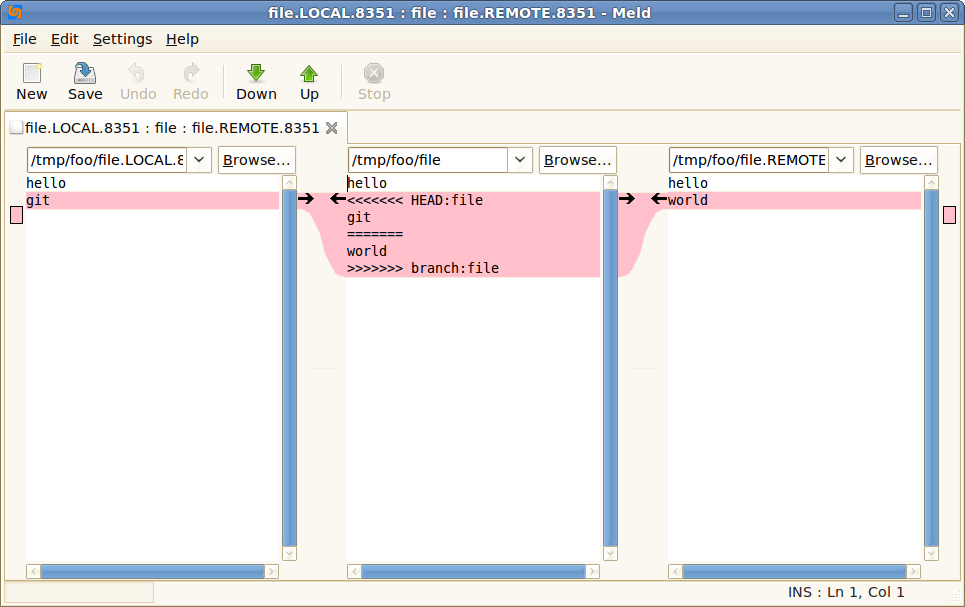
\includegraphics[width=11.5cm]{meld}};}
  \end{tikzpicture}
\end{frame}

\begin{frame}
  \frametitle{Getting out of trouble}
  \begin{description}[\texttt{git reset --hard \textit{commit}}]
  \item[\texttt{git reflog}] Show the \emph{reflog} entries for
    \texttt{HEAD}.
  \item[\texttt{git reflog show \textit{ref}}] Show the \emph{reflog}
    entries for \texttt{\textit{ref}}.
  \item[\texttt{git reset --hard \textit{commit}}] Resets the
    \emph{ref} pointed to by \texttt{HEAD}, as well as the index and
    working tree, to \texttt{\textit{commit}}.
  \end{description}

  \begin{itemize}
  \item The reflog tracks all local changes to refs.  Whenever a ref
    is updated to point at a new commit, it gets an entry in the
    reflog.
  \item If you find yourself somewhere you don't expect, you can
    examine the log or the reflog, and then use \texttt{reset} to get
    back to a known point.
  \item This works even in a conflicted merge or rebase, if you just
    want to bail out and try something different.
  \end{itemize}

\end{frame}

\begin{frame}[fragile]
  \frametitle{A peek at the reflog}
  {\footnotesize
  \begin{semiverbatim}
\sh{git reflog show master}
fc8da7a... master@{0}: commit (merge): Merge branch 'andersk'
994be80... master@{1}: merge andersk: Merge made by recursive.
383c158... master@{2}: commit: 6 is a number too.
4172330... master@{3}: commit (initial): 1, 2, 3, 4, 5!
\sh{git reflog show andersk}
5360c2d... andersk@{0}: commit: 5\textonehalf is a better number.
7aeb494... andersk@{1}: commit: Numbers start at 0.
4172330... andersk@{2}: branch: Created from HEAD
  \end{semiverbatim}}
\end{frame}

\section{Collaboration with Git}

\begin{frame}
  \frametitle{Collaboration with Git}
  \begin{itemize}
  \item Git allows bidirectional communication between any pair of
    repositories.
  \item Git speaks many protocols.
    \begin{itemize}
    \item SSH
    \item HTTP/HTTPS
    \item DAV
    \item Git protocol
    \item rsync
    \item direct filesystem access
    \end{itemize}
  \item This flexibility lets you implement a wide range of
    centralized or distributed development models.
  \end{itemize}
\end{frame}

\begin{frame}
  \frametitle{The simple case}

  \begin{itemize}
  \item A freshly cloned repository has one remote called
    \texttt{origin}, which is the default source for pulls and
    destination for pushes.
  \end{itemize}

  \begin{description}[\texttt{git branch -r}]
  \item[\texttt{git fetch}] Download commits from \texttt{origin}.
    Each remote branch \texttt{\textit{branch}} will be made available
    with the name \texttt{origin/\textit{branch}}.
  \item[\texttt{git branch -r}] List the available remote branches.
  \item[\texttt{git branch -a}] List the available local and remote branches.
  \end{description}

  \begin{itemize}
  \item Development is done on local branches.  To work on a remote
    branch, you first create a local \emph{tracking branch}, and then
    push any changes back to the remote branch as a separate
    operation.
  \end{itemize}
\end{frame}

\begin{frame}
  \frametitle{Tracking branches}

  \begin{description}[git pull --rebase]
  \item[\texttt{git checkout -b \textit{branch}
      origin/\textit{branch}}] Create and switch to a new tracking
    branch named \texttt{\textit{branch}}, set up to track the remote
    branch \texttt{origin/\textit{branch}}.
  \item[\texttt{git pull}] Update the current tracking branch from
    \texttt{origin/\textit{branch}}.  Short for \texttt{git fetch; git
      merge origin/\textit{branch}}.
  \item[\texttt{git pull --rebase}] Short for \texttt{git fetch; git
      rebase origin/\textit{branch}}.
  \item[\texttt{git push}] Push the current tracking branch back to
    \texttt{origin/\textit{branch}}.  This will only fast-forward the
    remote branch by default, so you may need to \texttt{git pull}
    first.
  \item[\texttt{git push origin :\textit{branch}}] Delete the remote
    branch \texttt{\textit{branch}}.
  \item[\texttt{git remote prune origin}] Clean up any refs to
    branches that have been deleted remotely.
  \end{description}
\end{frame}

\begin{frame}[fragile]
  \frametitle{Remotes}
  \begin{itemize}
  \item A Git repository can be configured with references to any
    number of \emph{remotes}.
  \item By default, a newly cloned repository has one remote named
    \texttt{origin} pointing to the source of the clone.
  \end{itemize}
  \begin{footnotesize}
\begin{semiverbatim}
\sh{git clone /mit/andersk/Public/git/nss_nonlocal.git}
Initialized empty Git repository in /tmp/nss_nonlocal/.git/
\sh{cat nss_nonlocal/.git/config}
\dots
[remote "origin"]
	url = /mit/andersk/Public/git/nss_nonlocal.git
	fetch = +refs/heads/*:refs/remotes/origin/*
[branch "master"]
	remote = origin
	merge = refs/heads/master
\end{semiverbatim}
  \end{footnotesize}
\end{frame}

\section{Rewriting history}

\begin{frame}
  \frametitle{Rewriting history}

  \begin{itemize}
  \item Git includes powerful tools for rewriting history.
  \item Of course, since modifying a commit changes its SHA-1
    identifier, by ``rewriting history'' we actually mean
    ``transforming a sequence of commits into a different sequence of
    commits''.
  \item You need to be careful about rewriting commits that others may
    have already pulled.
    \begin{itemize}
    \item By default, Git will prevent you from pushing changes that
      are not fast-forwards, unless you ask very hard.
    \end{itemize}
  \item Rewriting is extremely useful for cleaning up a private branch
    before making it publicly available.
  \end{itemize}
\end{frame}

\begin{frame}
  \frametitle{Why rewriting is useful}

  \begin{itemize}
  \item A good history will include one commit for each self-contained
    logical change to the tree.
  \item Avoid cluttering the history with typos and trivial bugs that
    are fixed in the following commits.
    \begin{itemize}
    \item This makes things more pleasant for anyone who wants to read
      or review your changes.
    \item It also makes it easier to pinpoint bugs with \texttt{git
        bisect}.
    \end{itemize}
  \item You don't need to worry about making your commits perfect as
    you write them, since you can rearrange them later.
  \end{itemize}
\end{frame}

\begin{frame}
  \frametitle{Resetting branches}

  \begin{description}[\texttt{git reset --hard \textit{commit}}]
  \item[\texttt{git reset --hard \textit{commit}}] Resets the current
    \texttt{HEAD}, as well as the index and working tree, to
    \texttt{\textit{commit}}.
  \item[\texttt{git reset \textit{commit}}] Resets the current
    \texttt{HEAD} and index to \textit{commit}, without touching the
    working tree.
  \item[\texttt{git reset --soft \textit{commit}}] Resets the current
    \texttt{HEAD} to \textit{commit}, without touching the index or
    the working tree.
  \item[\texttt{git commit --amend}] Adds the modifications in the
    index to the current commit at \texttt{HEAD} ``in place''.
    Approximately equivalent to \texttt{git reset
      HEAD\textasciicircum; git commit}.
  \end{description}
\end{frame}

\begin{frame}
  \frametitle{Rebasing}
  \begin{description}[\texttt{git rebase \textit{commit}}]
  \item[\texttt{git rebase \textit{commit}}] Rebase \texttt{HEAD} onto
    \texttt{\textit{commit}}.
  \end{description}

  \begin{itemize}
  \item \texttt{rebase} finds all commits that are in \texttt{HEAD}
    but not in \texttt{\textit{commit}}, and re-applies them starting
    with \texttt{\textit{commit}}. The current branch is reset to the
    result.
  \item This has a similar effect to a merge, but maintains a linear
    history, at the cost of losing some information.
  \item \texttt{rebase} \emph{changes the object identifiers} of the
    re-applied commits.
  \item \texttt{rebase} is often preferred to keep history clean.
  \end{itemize}
\end{frame}

\begin{frame}
  \frametitle{Rebase vs.\ merge}
  \begin{itemize}
  \only<1>{\item We have development on both a \emph{topic branch} and
    \texttt{master}.}
  \only<2>{\item \texttt{merge} results in a forked history:}
  \only<3>{\item \texttt{rebase} rewrites commits and maintains a
    linear history:}
  \end{itemize}
    \begin{center}
    \only<1>{\includegraphics[width=5cm]{rebase1}}
    \only<2>{\includegraphics[width=5cm]{rebase2}}
    \only<3>{\includegraphics[width=5cm]{rebase3}}
  \end{center}
\end{frame}

\begin{frame}
  \frametitle{Interactive rebasing}
  \begin{description}[\texttt{git rebase -i \textit{commit}}]
  \item[\texttt{git rebase -i \textit{commit}}] Rebase \texttt{HEAD}
    onto \texttt{\textit{commit}}, letting you interactively edit the
    resulting history.
  \end{description}

  \begin{itemize}
  \item Git will start your editor on a list of the commits to be
    applied on top of \textit{commit}.
  \item You can cut and paste to arbitrarily reorder the commits.
  \item You can delete a line to remove that commit completely.
  \item You can insert the \texttt{squash} directive to fuse a commit
    into the previous commit.
  \item You can insert the \texttt{edit} directive to have Git pause
    after applying a commit, so you can amend it in place or insert
    new commits, before further commits are applied.
  \end{itemize}
\end{frame}

\begin{frame}
  \frametitle{And beyond!}

  \begin{description}[\texttt{git filter-branch}]
  \item[\texttt{git bisect}] Easily pinpoint a regression in your
    history using a repeated bisection search.
  \item[\texttt{git cvsimport}, \texttt{git svn}] Use Git to work with
    repositories in other formats.  (I think Git makes a much better
    CVS or SVN client than the native ones!)
  \item[\texttt{git filter-branch}] Rewrite history by mapping each
    commit through an arbitrary script.
  \item[\texttt{git format-patch}, \texttt{git send-email}, \text{git
      am}] Send and receive Git patches by email.
  \item[\texttt{git stash}] Quickly stash away and reapply temporary
    changes while you do other work.
  \item[\texttt{git submodule}] Manage a group of related Git
    repositories.
  \item[\texttt{gitk}] A graphical repository browser that's great for
    visualizing how your actions affect the state of your repository.
  \end{description}
\end{frame}

\begin{frame}
  \frametitle{Exploring Git yourself}

  \begin{itemize}
  \item There are many commands we haven't talked about, and the ones
    we have take additional options that can help you work more
    efficiently.
  \item Anything you think you should be able to do within the Git
    model can probably be done.
  \item Git is designed to be conveniently scriptable.
  \item Git has extensive documentation---start with \texttt{man git}.
    \begin{itemize}
    \item To get documentation on any \texttt{git \textit{command}},
      run \texttt{git help \textit{command}} or (equivalently)
      \texttt{man git-\textit{command}}.
    \end{itemize}
  \end{itemize}
\end{frame}

\end{document}
